\section{Le moteur physique}

\subsection{Algorithme général}

Nous disposons désormais des briques de base nécessaires à la
construction de l'algorithme général du moteur physique. Un appel à
cette procédure intégrera les états de tous les corps de la simulation
d'un pas de temps $\deriv t$ en tenant compte des interactions
possibles. On part de l'hypothèse que tous les corps sont initialement
séparés et donc qu'aucune interpénétration ne se produit au départ.

En premier lieu, on vérifie pour chaque paire de corps s'ils entrent
en collision. Si tel est le cas, on corrige leur état puis on applique
les impulsions adaptées. Ensuite, on administre des forces
environnementales, telles que la gravité. Il ne reste plus qu'à
intégrer l'état de tous les corps, c'est à dire mettre à jour leurs
position et orientation en fonction des élans transmis par les
impulsions et les forces extérieures. L'algorithme \ref{algoMoteur1}
résume cette organisation.

\begin{algorithm}[h]
  \caption{Boucle principale}
  \label{algoMoteur1}
  \dontprintsemicolon
  \SetKwData{pairedecorps}{paire de corps}
  \SetKwData{contact}{contact}
  \SetKwData{corps}{corps}
  \SetKwFunction{collisionGrossiere}{collisionGrossiere}
  \SetKwFunction{collisionFine}{collisionFine}
  \SetKwFunction{corrigerCollision}{corrigerCollision}
  \SetKwFunction{detecterContacts}{detecterContacts}
  \SetKwFunction{calculerImpulsion}{calculerImpulsion}
  \SetKwFunction{appliquer}{appliquer}
  \SetKwFunction{appliquerForcesEnvironnementales}{appliquerForcesEnvironnementales}
  \SetKwFunction{integrer}{integrer}
  \Entree{Un pas de temps $\deriv t$}
  \BlankLine
  \PourCh{\pairedecorps (A,B)}{
    \Si{\collisionGrossiere{A,B}}{
      \Si{\collisionFine{A,B}}{
        \corrigerCollision{A,B}\;
        $C \leftarrow$ \detecterContacts{A,B}\;
        \PourCh{\contact $c \in C$}{
          $I \leftarrow$ \calculerImpulsion{c}\;
          \appliquer{I, A}\;
          \appliquer{-I, B}\;
        }
      }
    }
  }
  \BlankLine
  \PourCh{\corps A}{
    \appliquerForcesEnvironnementales{A}\;
    \integrer{A, $\deriv t$}
  }
  \BlankLine
\end{algorithm}

Cette structure simple fonctionne de façon satisfaisante lorsque la
simulation comporte peu d'objets. Néanmoins, sa stabilité est
fortement compromise lorsque de nombreux corps entrent en jeu et ce,
pour plusieurs raisons.

Depuis le début de la conception du moteur physique, nous détectons,
corrigeons et traîtons les collisions entre paire de corps. On part de
l'hypothèse qu'au début de la simulation aucun solide n'entre en
collision avec un autre et grâce à la phase de correction
collisionnelle, cette hypothèse est vérifiée au début de chaque
intégration. Un problème majeur de l'algorithme actuel est qu'il
provoque des situation d'interpénétration non corrigeables, notamment
lorsque des amas d'objets se forment. La sous-figure $a$ de la figure
\ref{probleme} prend place au début d'une itération de la simulation.
On y voit un corps $A$, attiré par la gravité, et s'étant enfoncé dans
le sol. Le corps $B$ subit quand à lui la même influence mais ne tombe
pas assez bas pour qu'une collision avec $A$ s'opère. La sous-figure
$b$ nous montre le résultat de la correction de l'interpénétration
entre $A$ et le sol et on remarque qu'une nouvelle collision entre $B$
et $A$ en découle. L'issue de cette situation dépend de $B$; si sa
phase de détection de collision est déjà passée alors il est déjà trop
tard et $A$ et $B$ seront en état d'interpénétration à l'itération
suivante et l'hypothèse de non-pénétration ne sera pas respectée. Le
comportement de la simulation sera alors imprévisible. La stabilité du
moteur physique est donc gravement dépendante de l'ordre arbitraire
dans lequel les corps sont rangés et exécutent leur détection de
collision.

\begin{figure}
  \centering
  \subfloat[]{ \begin{tikzpicture}[scale=0.4,transform shape]
  \draw[black,thick] (0,0) -- (10,0);

  \draw[->,thick,black,font=\huge] (1,5) to node[black,auto,swap] {$\vec{G}$} (1,1);

  \node[
    rectangle,
    minimum width=5cm,
    minimum height=4cm,
    draw=bleu,
    thick] at (5,1) (a) {};

  \node[
    rectangle,
    minimum width=6cm,
    minimum height=2cm,
    draw=rose,
    thick] at (5,4.5) (b) {};

\end{tikzpicture}
 }
  \subfloat[]{ \begin{tikzpicture}[scale=0.35,transform shape]
  \draw[black,thick] (0,0) -- (10,0);


  \node[
    rectangle,
    minimum width=5cm,
    minimum height=4cm,
    draw=bleu,
    thick] at (5,2.1) (a) {};

  \node[
    rectangle,
    minimum width=6cm,
    minimum height=2cm,
    draw=rose,
    thick] at (5,4.5) (b) {};

  \node[
    rectangle,
    minimum height=1cm] at (0,-0.53) (s) {};

\end{tikzpicture}
 }
  \caption{Interpénétration collatéralement provoquée par une correction collisionnelle}
  \label{probleme}
\end{figure}

De plus, l'organisation actuelle prive la simulation de toute
cohérence temporelle. En effet, à chaque itération tous les corps
avancent d'un pas de temps fixe $\deriv t$ mais l'état de ceux
subissant une collision sera inmanquablement corrigé pour correspondre
à l'état qu'ils auraient dû atteindre au moment du contact. On se
retrouve ainsi avec des corps n'ayant pas subi de collision, côtoyant
des corps en ayant subit et dont l'état correspond à un temps
précédent.

Autre problème de taille : la simulation empruntera des chemins
différents selon l'ordre dans lequel les collisions sont détectées. La
figure \ref{issues} nous montre deux corp ainsi que la position qu'ils
atteindraient à l'itération suivante si l'on ignorait les collisions
(en pointillés). On peut aisément se rendre compte des conséquences de
l'ordre dans lequel les objets sont traîtés. Si le corps bleu est
traîté en premier, il entrera en collision avec le corps rose, son
état sera corrigé, et une impulsion sera plus tard générée pour
séparer les deux corps. Au final, l'objet bleu sera projeté vers la
gauche et le corps rose sera dévié de sa trajectoire originelle. Par
contre, si c'est le corps rose qui est traîté en premier, il avancera
vers sa prochaine position, puis ce sera autour de l'autre corps de se
déplacer. Puisque le corps rose ne se trouvera plus sur sa
trajectoire, rien ne se passera !

\begin{figure}
  \centering
  \subfloat{ \begin{tikzpicture}[scale=0.9,transform shape]
  \coordinate (A1) at (0,0);
  \coordinate (A2) at (4.2,0);
  \coordinate (B1) at (5,0);
  \coordinate (B2) at (5,-3);

  \node[
    circle,
    minimum size=1cm,
    draw=bleu,
    thick] at (A1) (a1) {};
  \node[
    circle,
    minimum size=1cm,
    draw=bleu,
    thick,
    dotted] at (A2) (a2) {};
  \draw[->,thick,vert,font=\large] (A1) to node[black,auto] {$+ \deriv t$} (A2);

  \node[
    circle,
    minimum size=1cm,
    draw=rose,
    thick] at (B1) (b1) {};
  \node[
    circle,
    minimum size=1cm,
    draw=rose,
    thick,
    dotted] at (B2) (b2) {};
  \draw[->,thick,vert,font=\large] (B1) to node[black,auto] {$+ \deriv t$} (B2);

\end{tikzpicture}
 }
  \caption{Deux issues possibles selon l'ordre du traitement des collisions}
  \label{issues}
\end{figure}

Tous les problèmes cités sont clairement liés à un manque de cohérence
temporelle. Lors de l'utilisation d'un tel algorithme, on utilise un
pas de temps dit explicite \cite{garstenauer}. Nous allons maintenant
nous tourner vers une version améliorée, dont le pas de temps sera dit
implicite.

L'algorithme \ref{algoMoteur2} est plus solide dans la mesure o\`u il
détecte à chaque itération le temps du premier contact et intègre tous
les corps de la simulation jusqu'à cet instant de façon à traîter les
collisions dans leur ordre réel. Détaillons le fonctionnement de cette
nouvelle méthodologie. En premier lieu, on copie chaque corps afin de
s'assurer que les modifications qui vont suivre ne changent pas leur
véritable état de départ. On avance ensuite l'état de chaque copie
pour détecter si une collion se produira avec l'autre. Si tel est le
cas, on corrige la pénétration et on détermine les informations de
contact. \`A la fin de cette phase de prédiction, on dispose d'une
liste de contacts potentiels qu'il est nécessaire de trier en fonction
du temps d'impact. On intègre l'état de tous les objets d'un pas de
temps égal au plus faible temps d'impact.

\begin{algorithm}[h]
  \caption{Boucle principale améliorée}
  \label{algoMoteur2}
  \dontprintsemicolon
  \SetKwData{pairedecorps}{paire de corps}
  \SetKwData{contact}{contact}
  \SetKwData{corps}{corps}
  \SetKwFunction{collisionGrossiere}{collisionGrossiere}
  \SetKwFunction{collisionFine}{collisionFine}
  \SetKwFunction{corrigerCollision}{corrigerCollision}
  \SetKwFunction{detecterContacts}{detecterContacts}
  \SetKwFunction{calculerImpulsion}{calculerImpulsion}
  \SetKwFunction{appliquer}{appliquer}
  \SetKwFunction{integrer}{integrer}
  \SetKwFunction{trierContacts}{trierContacts}
  \SetKwFunction{appliquerForcesEnvironnementales}{appliquerForcesEnvironnementales}
  \SetKwFunction{mint}{min}
  \Entree{Un pas de temps $\deriv t$}
  \BlankLine
  $C \leftarrow \emptyset$\;
  \PourCh{\pairedecorps (A,B)}{
    $A_2 \leftarrow A$\;
    $B_2 \leftarrow B$\:
    \appliquerForcesEnvironnementales{$A_2$}\;
    \integrer{$A_2$, $\deriv t$}
    \appliquerForcesEnvironnementales{$B_2$}\;
    \integrer{$B_2$, $\deriv t$}
    \BlankLine
    \Si{\collisionGrossiere{$A_2$, $B_2$}}{
      \Si{\collisionFine{$A_2$, $B_2$}}{
        \corrigerCollision{$A_2$, $B_2$}\;
        $C \leftarrow C \cup$ \detecterContacts{$A_2$, $B_2$}\;
      }
    }
  }
  \BlankLine
  \trierContacts{C}\;
  $\deriv t_2 \leftarrow$ \mint{$\deriv t$, C[0].t} 
  \BlankLine
  \PourCh{\corps A}{
    \appliquerForcesEnvironnementales{A}\;
    \integrer{A, $\deriv t_2$}
  }
  \BlankLine
  \PourCh{\contact $c \in C | c.t = \deriv t_2$}{
    $I \leftarrow$ \calculerImpulsion{c}\;
    \appliquer{I, A}\;
    \appliquer{-I, B}\;
  }
  \BlankLine
\end{algorithm}

Ce nouvel algorithme assure la cohérence temporelle car les corps sont
maintenant tous intégrés à l'aide du même pas de temps à chaque
itération. De plus l'ordre des collisions est respecté puisqu'on se
limite au traitement de celles apparaissant le plus tôt. Il se révèle
tout de même moins économique que son prédécesseur dans la mesure o\`u
l'on intègre chaque corps non pas une fois, mais $\frac{n(n-1)}{2}$
fois, avec $n$ le nombre d'objets de la simulation. Ce coût
supplémentaire est nécessaire si l'on veut obtenir des informations de
contact isolées à une paire de corps et ignorant les autres objets.

\subsection{Démonstrations}

\subsubsection*{Simulation basique}

Commençons par mettre en place une simulation basique faisant
intervenir la gravité. Un cube est fixé sur une plate-forme et on fait
apparaître une boîte à quelques mètres de hauteur. Observons son
comportement (figure \ref{demoBox}).

\begin{figure}
  \centering
  \subfloat[La boîte dispose initialement d'une vitesse
    nulle mais accélère rapidement vers le bas sous l'influence de la
    gravité. Elle rentre en contact avec le cube.]{
    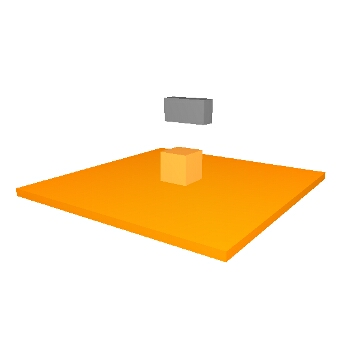
\includegraphics[width=2.5cm]{images/screenshots/box/1.jpg}
    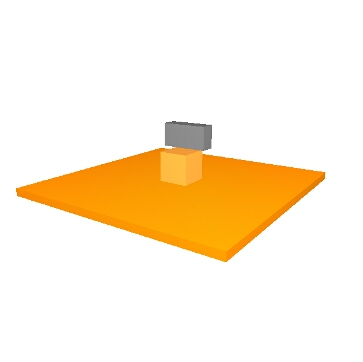
\includegraphics[width=2.5cm]{images/screenshots/box/2.jpg}
    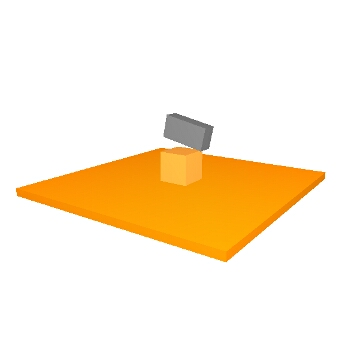
\includegraphics[width=2.5cm]{images/screenshots/box/3.jpg}
  }
  \qquad
  \subfloat[La boîte rebondit sur le cube. Comme les points de
    contact sont excentrés par rapport à son centre de masse, une
    rotation s'en suit.]{
    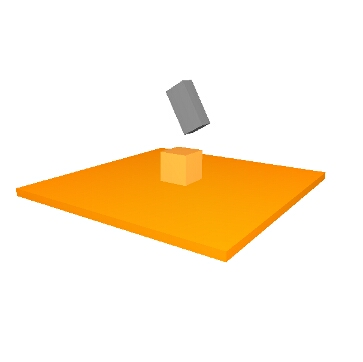
\includegraphics[width=2.5cm]{images/screenshots/box/4.jpg}
    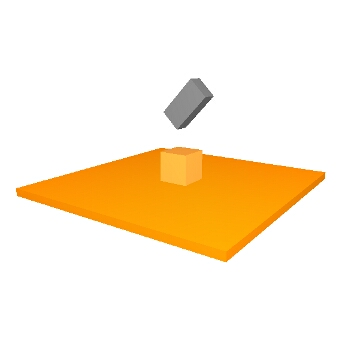
\includegraphics[width=2.5cm]{images/screenshots/box/5.jpg}
    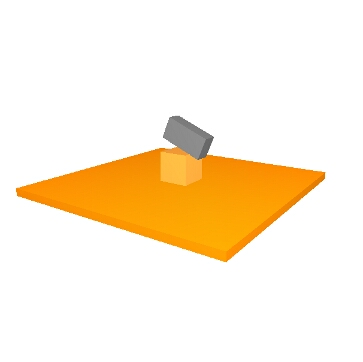
\includegraphics[width=2.5cm]{images/screenshots/box/6.jpg}
  }
  \qquad
  \subfloat[La boîte rebondit à nouveau sur le cube. Cette fois
    ci, sa vitesse angulaire la projette vers l'extérieur.]{
    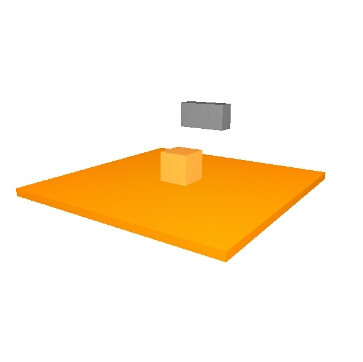
\includegraphics[width=2.5cm]{images/screenshots/box/7.jpg}
    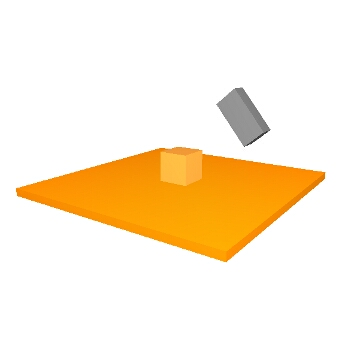
\includegraphics[width=2.5cm]{images/screenshots/box/8.jpg}
    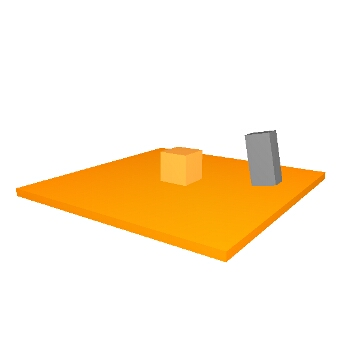
\includegraphics[width=2.5cm]{images/screenshots/box/9.jpg}
  }
  \qquad
  \subfloat[La boîte entre en collision avec le sol et rebondit
    pour finir sa course dans le vide.]{
    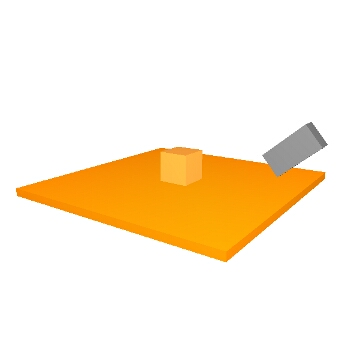
\includegraphics[width=2.5cm]{images/screenshots/box/10.jpg}
    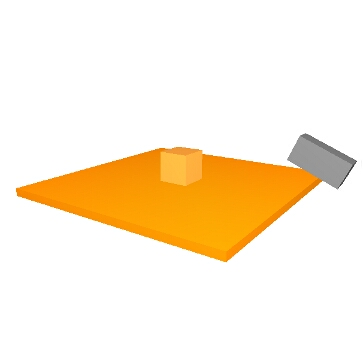
\includegraphics[width=2.5cm]{images/screenshots/box/11.jpg}
  }
  \caption{}
  \label{demoBox}
\end{figure}

\subsubsection*{Pachinko}

Le pachinko est un jeu de hasard japonais dans lequel des billes
métalliques sont lachées dans un parcours vertical parsemé de petites
tiges les déviant de leur trajectoire. Selon le chemin qu'elles
empruntent, de nouvelles billes peuvent être remportées, à la manière
d'une machine à sous.

Utilisons l'exemple de la machine à Pachinko pour illustrer les
capacités de notre moteur physique.

\subsection{Perspectives d'évolution}

\subsubsection{Tunneling}

Le moteur physique que nous concevons fonctionne par intégration
discrète et si aucun contrôle n'est effectué pour contrecarrer les
effets négatifs de cette caractéristique, on risque d'obtenir des
résultats imprécis ou pire, complètement éloignés de ce que l'on
retrouverait dans la réalité. On a par exemple vu plus tôt qu'une
phase de recherche dichotomique est nécessaire pour recaler les corps
à leur position réelle de contact lorsqu'une collision est détectée.

Néanmoins, une éventualité n'a pas été envisagée : que se passerait-il
si un objet en traversait entièrement un autre pendant un pas de temps
? On peut imaginer un objet $A$ lancé vers un autre objet $B$
fixe. \`A l'instant $t$, $A$ n'entre pas en collision avec $B$ mais se
dirige dans sa direction. \`A l'instant $t + \deriv t$, $A$ a
entièrement traversé $B$. \`A aucun de ces deux instants une collision
n'a été détectée et pourtant $A$ est impunément passé à travers
$B$. Le pas de temps utilisé pour réguler l'intégration du système
était donc trop faible pour s'assurer des collisions entre corps
évoluant à haute vitesse. Ce phénomène est appelé
\textit{tunneling}. \`A l'heure de l'écriture de ce rapport, le moteur
physique est sensible à ce genre de situation. Réellement, ce cas ne
se produit pas, puisque les simulations développées représentent des
situations terrestres qui font participer des forces d'opposition
telles que le frottement de l'air et donc les corps n'atteignent
jamais de vitesses démesurées. On souhaite tout de même disposer d'un
moteur physique solide et versatile, évaluons les possibilités qui
s'offrent à nous pour pallier ce problème.
\begin{figure}
  \centering
  \begin{tikzpicture}[scale=0.7, transform shape]
  \coordinate (AT1) at (0,0);
\coordinate (AT2) at (8,0);
\coordinate (B) at (6,0);

\draw node[fig,
  circle,
  minimum size=2cm,
  draw=bleu,
  dotted] (a1) at (AT1) {};

\node[fig,
  circle,
  minimum size=2cm,
  draw=bleu] (a2) at (AT2) {};
\node[fig,
  circle,
  minimum size=1cm,
  draw=rose] (b) at (B) {};



  \draw[->,thick,vert] (AT1) to node[black,auto] {$\deriv t$} (AT2);
\end{tikzpicture}

  \caption{Le phénomène du tunneling}
  \label{tunneling1}
\end{figure}

On pourrait envisager de diminuer la durée du pas de temps
d'intégration afin de diminuer le risque de tunneling, mais même si un
pas de temps faible améliore la qualité des résultats, il ne pourra
pas être indéfiniment réduit. Il est principalement limité par le
temps de calcul d'une mise à jour du système, puisqu'à partir du
moment o\`u $\deriv t$ est inférieur au temps moyen nécessaire à une
machine pour calculer une itération de la simulation, le programme
perdra son statut d'application temps réel.

Une technique usuellement admise est le lancer de rayons
(\textit{raycasting}) entre les points de la position de départ du
solide et les points de sa position d'arrivée. Si l'un des rayons
touche un autre corps, on sait qu'une collision aurait dû être
détectée et on peut revenir en arrière. Cette méthode présente
pourtant une faiblesse de taille, car le résultat de cette recherche
dépend directement de la concentration de rayons. Si on lance peu de
rayons, on risque de ne pas détecter les corps de petite taille et
donc de les traverser tandis qu'une concentration élevée de rayons
pourrait se réveler regrettable en terme de coûts de calcul.

\begin{figure}
  \centering
  \begin{tikzpicture}[scale=0.7, transform shape]
  \coordinate (AT1) at (0,0);
\coordinate (AT2) at (8,0);
\coordinate (B) at (6,0);

\draw node[fig,
  circle,
  minimum size=2cm,
  draw=bleu,
  dotted] (a1) at (AT1) {};

\node[fig,
  circle,
  minimum size=2cm,
  draw=bleu] (a2) at (AT2) {};
\node[fig,
  circle,
  minimum size=1cm,
  draw=rose] (b) at (B) {};



  \path[rayon] (a1.north) -- (a2.north);
  \path[rayon] (a1.west) -- (a2.west);
  \path[rayon] (a1.north west) -- (a2.north west);
  \path[rayon] (a1.south) -- (a2.south);
  \path[rayon] (a1.south west) -- (a2.south west);
\end{tikzpicture}

  \caption{Lancer de rayons pour la détection de tunneling}
  \label{tunneling2}
\end{figure}

La technique de la détection de collision continue (\textit{continuous
  collision detection}) permet de contrôler de façon certaine tout
phénomène de tunneling. L'idée est la suivante : soit deux corps $A$
et $B$ dont l'on veut détecter l'éventuelle collision. On construit
deux volumes fantômes $C_A$ et $C_B$ englobant tous les points par
lesquels passent respectivement $A$ et $B$ entre deux
intégrations. Ces volumes n'interviendront pas dans les collisions des
autres objets de la simulation, et on vérifie simplement s'ils entrent
tous deux en collision. Si tel est le cas, alors on sait qu'il est
possible qu'un tunneling se soit produit et on peut revenir en arrière
jusqu'à ce que le problème soit résolu. Pour accélérer cette phase, il
est envisageable d'utiliser des boîtes englobantes de la même façon
que lors de la détection grossière de collision. L'un des avantages
majeurs de cette méthode, en plus de sa certitude de ne manquer aucun
tunneling, est sa simplicité de mise en place puisque toutes les
routines de détection et de retour en arrière utilisées ont déjà été
écrites et entrent en jeu dans le fonctionnement de base du moteur
physique.

\begin{figure}
  \centering
  \begin{tikzpicture}[scale=0.7, transform shape]
  \coordinate (AT1) at (0,0);
\coordinate (AT2) at (8,0);
\coordinate (B) at (6,0);

\draw node[fig,
  circle,
  minimum size=2cm,
  draw=bleu,
  dotted] (a1) at (AT1) {};

\node[fig,
  circle,
  minimum size=2cm,
  draw=bleu] (a2) at (AT2) {};
\node[fig,
  circle,
  minimum size=1cm,
  draw=rose] (b) at (B) {};



  \coordinate (a1n) at ($(a1.north)+(0,0.2)$);
  \coordinate (a2s) at ($(a2.south)+(0,-0.2)$);

  \draw[gris] (a1n) arc (90:270:1.2cm) --
  (a2s) arc (-90:90:1.2cm) --
  (a1n);
\end{tikzpicture}

  \caption{Boîtes englobantes pour la détection de tunneling}
  \label{tunneling3}
\end{figure}

\subsubsection{Partitionnement de l'espace}

Comme mis en avant tout au long de ce rapport, on cherche à concevoir
un moteur physique dont la rapidité d'éxécution est un facteur
déterminant. Dans cette optique, il est primordial d'optimiser les
routines géométriques entrant en jeu mais aussi d'éviter leur
exécution inutile dès que possible. La détection des collisions entre
les corps qui peuplent notre système se déroule en deux étapes : une
détection grossière visant à vérifier de façon économique si deux
objets se touchent et une détection fine servant à confirmer ou à
infirmer de façon sûre ce résultat. Bien que la détection grossière
soit peu coûteuse en termes de calcul, elle est éxécutée pour $n$
corps au minimum $\frac{n(n-1)}{2}$ fois à chaque itération, et ce
sans compter les détections de collision exécutées pendant la
recherche dichotomisuqe de l'état de contact. Pourtant, il est très
souvent inutile de détecter si deux objets sont en situation
d'interpénétration, par exemple lorsque la distance les séparant est
grande. Il serait tout à notre avantage d'ajouter au moteur une couche
supplémentaire tenant compte de ces disparités spatiales pour
accélérer la phase de détection de collision.

Le principe général du partitionnement de l'espace (\textit{spatial
  partitioning}) est de subdiviser l'environnement de la simulation en
sous-espaces. La répartition des corps dans ces sous-espaces dépend
bien évidemment de leur position dans le repère global mais aussi du
volume qu'ils occupent. On est certain que seules les entités
appartenant à un même sous-espace peuvent interagir entres elles, on
dispose donc d'une aide quant au choix des objets entre lesquels
vérifier si collision il y a.

Sous sa forme la plus simple, le partitionnement de l'espace prend la
forme d'une grille de taille fixe dans les cases de laquelle les corps
de la simulation sont répartis. L'aspect statique d'une telle
structure présente plusieurs inconvénients majeurs, notamment le fait
que le gain de performance variera fortement selon le nombre d'objets
considérés, leur taille et la finesse de la grille. Par exemple, si
une grille a des cases trop grandes, chacune contiendra de nombreux
objets et le gain de performance sera peu flagrant. Si au contraire
les cases de la grille sont trop petites, les plus grands objets ne
pourront pas rentrer dans leur intégralité à l'intérieur d'une unique
case. Une solution à ce problème est de ranger un même objet dans
plusieurs cases adjacentes de la grille, mais une fois encore, si des
corps sont démultipliés de la sorte, le temps de maintenance d'une
telle structure sera augmenté.

Une variante plus subtile de partitionnement de l'espace est
l'utilisation d'\textit{octrees} (\textit{quadtrees} en deux
dimensions) \cite{millington}. Cette structure de données prend la forme d'un arbre
représentant l'espace à subdiviser. Chaque n\oe ud de l'arbre possède
huit fils, chacun correspondant à un octant du volume de leur père. La
racine de l'arbre est associée au volume complet de l'environnement
que l'on souhaite diviser. Lorsqu'un corps est introduit dans la
simulation, il faut le ranger dans l'arbre. Pour ce faire, on part de
la racine et on descend récursivement jusqu'à une feuille de l'arbre
en se guidant dans les embranchements selon la position et le volume
de l'objet à insérer. L'octree n'est pas nécessairement équilibré et
plus une zone contient de corps et plus elle pourra être subdivisée.

Cette structure sert à stocker les corps de la simulation, et si nous
l'implémentions elle remplacerait la liste qui contient nos objets et
dont l'ordre est actuellement arbitraire. Elle devient
particulièrement intéressante lors de la phase de détection de
collision car il n'est plus désormais nécessaire de tester tous les
corps deux à deux; il suffit de vérifier les collisions entre les
corps du même sous-espace, autrement dit avec tous ceux contenus dans
la même feuille.
